\documentclass{standalone}
\usepackage{tikz}
\usetikzlibrary{patterns}
\usetikzlibrary{positioning}
\usetikzlibrary{patterns, positioning}
\usetikzlibrary{shapes.misc}
\usepackage[outline]{contour}
\contourlength{1.5pt} 
\usetikzlibrary{calc}
        \usepackage{relsize}
        \tikzset{fontscale/.style = {font=\relsize{#1}}}

\begin{document}
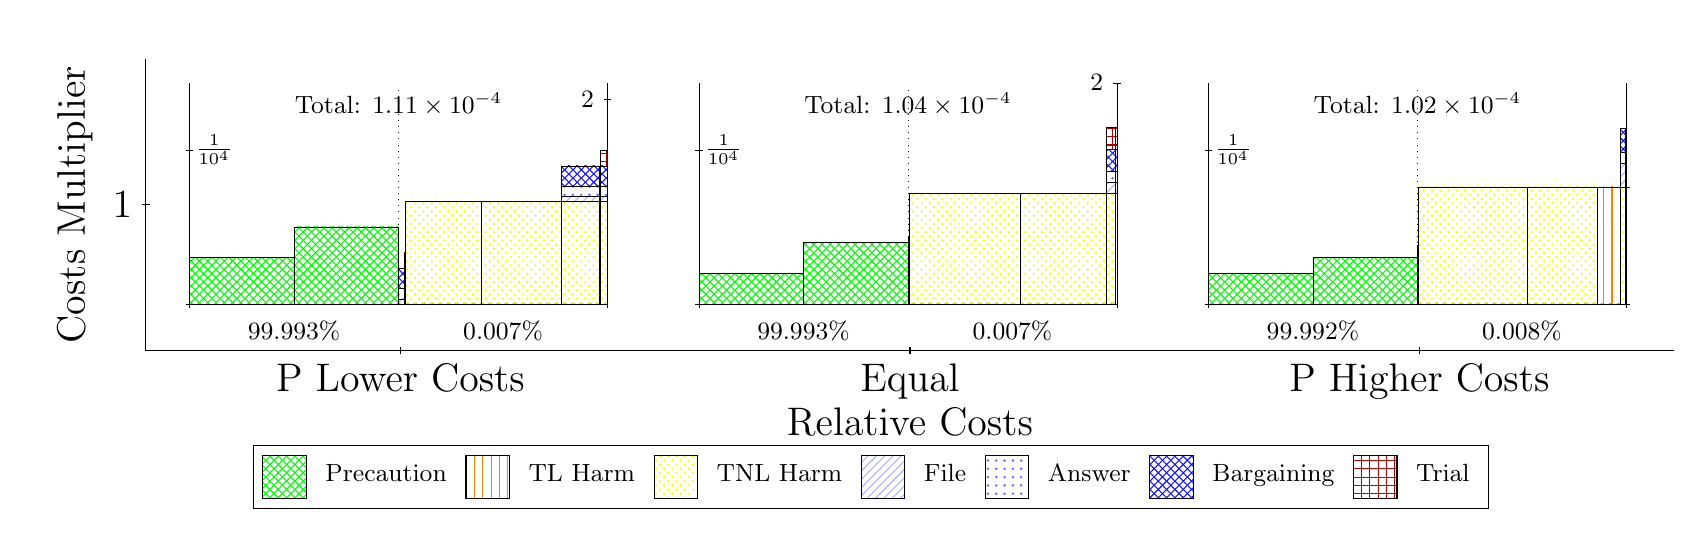
\begin{tikzpicture}
\clip(-0.5,-1.1) rectangle +(20.91,6.2);
\draw[black] (1,1) -- (1,4.7);
\node[rotate=90, fontscale=2, anchor=center] at (0.1, 2.85) {Costs Multiplier};
\draw[black] (0.95,2.85) -- (1.05,2.85);
\node[fontscale=2, anchor=east] at (0.95, 2.85) {1};

\draw[black] (1,1) -- (20.41,1);
\node[fontscale=2, anchor=center] at (10.705, 0.1) {Relative Costs};
\draw[black] (4.235,0.95) -- (4.235,1.05);
\node[fontscale=2, anchor=north] at (4.235, 0.95) {P Lower Costs};
\draw[black] (10.705,0.95) -- (10.705,1.05);
\node[fontscale=2, anchor=north] at (10.705, 0.95) {Equal};
\draw[black] (17.175,0.95) -- (17.175,1.05);
\node[fontscale=2, anchor=north] at (17.175, 0.95) {P Higher Costs};


\draw[pattern=crosshatch, pattern color=green,draw=black,very thin] (1.5556,1.592) rectangle (2.8828,2.1784);
\draw[pattern=crosshatch, pattern color=green,draw=black,very thin] (2.8828,1.592) rectangle (4.21,2.5693);
\draw[pattern=crosshatch, pattern color=green,draw=black,very thin] (4.21,1.592) rectangle (4.2765,1.592);
\draw[pattern=north east lines, pattern color=blue!30,draw=black,very thin] (4.21,1.592) rectangle (4.2765,1.6569);
\draw[pattern=dots,  pattern color=blue!60,draw=black,very thin] (4.21,1.6569) rectangle (4.2765,1.7867);
\draw[pattern=crosshatch,      pattern color=blue!90,draw=black,very thin] (4.21,1.7867) rectangle (4.2765,2.0462);
\draw[pattern=crosshatch, pattern color=green,draw=black,very thin] (4.2765,1.592) rectangle (4.2892,1.592);
\draw[pattern=north east lines, pattern color=blue!30,draw=black,very thin] (4.2765,1.592) rectangle (4.2892,1.6569);
\draw[pattern=dots,  pattern color=blue!60,draw=black,very thin] (4.2765,1.6569) rectangle (4.2892,1.7867);
\draw[pattern=crosshatch,      pattern color=blue!90,draw=black,very thin] (4.2765,1.7867) rectangle (4.2892,2.0462);
\draw[pattern=grid,            pattern color=red!70!black,draw=black,very thin] (4.2765,2.0462) rectangle (4.2892,2.2409);
\draw[pattern=crosshatch, pattern color=green,draw=black,very thin] (4.2892,1.592) rectangle (5.2549,1.592);
\draw[pattern=crosshatch dots, pattern color=yellow,draw=black,very thin] (4.2892,1.592) rectangle (5.2549,2.8897);
\draw[pattern=crosshatch, pattern color=green,draw=black,very thin] (5.2549,1.592) rectangle (6.2786,1.5921);
\draw[pattern=crosshatch dots, pattern color=yellow,draw=black,very thin] (5.2549,1.5921) rectangle (6.2786,2.8897);
\draw[pattern=crosshatch, pattern color=green,draw=black,very thin] (6.2786,1.592) rectangle (6.7652,1.592);
\draw[pattern=crosshatch dots, pattern color=yellow,draw=black,very thin] (6.2786,1.592) rectangle (6.7652,2.8897);
\draw[pattern=north east lines, pattern color=blue!30,draw=black,very thin] (6.2786,2.8897) rectangle (6.7652,2.9546);
\draw[pattern=dots,  pattern color=blue!60,draw=black,very thin] (6.2786,2.9546) rectangle (6.7652,3.0844);
\draw[pattern=crosshatch,      pattern color=blue!90,draw=black,very thin] (6.2786,3.0844) rectangle (6.7652,3.3439);
\draw[pattern=crosshatch, pattern color=green,draw=black,very thin] (6.7652,1.592) rectangle (6.7689,1.592);
\draw[pattern=vertical lines, pattern color=orange,draw=black,very thin] (6.7652,1.592) rectangle (6.7689,2.8897);
\draw[pattern=north east lines, pattern color=blue!30,draw=black,very thin] (6.7652,2.8897) rectangle (6.7689,2.9546);
\draw[pattern=dots,  pattern color=blue!60,draw=black,very thin] (6.7652,2.9546) rectangle (6.7689,3.0844);
\draw[pattern=crosshatch,      pattern color=blue!90,draw=black,very thin] (6.7652,3.0844) rectangle (6.7689,3.3439);
\draw[pattern=crosshatch, pattern color=green,draw=black,very thin] (6.7689,1.592) rectangle (6.8614,1.592);
\draw[pattern=crosshatch dots, pattern color=yellow,draw=black,very thin] (6.7689,1.592) rectangle (6.8614,2.8897);
\draw[pattern=north east lines, pattern color=blue!30,draw=black,very thin] (6.7689,2.8897) rectangle (6.8614,2.9546);
\draw[pattern=dots,  pattern color=blue!60,draw=black,very thin] (6.7689,2.9546) rectangle (6.8614,3.0844);
\draw[pattern=crosshatch,      pattern color=blue!90,draw=black,very thin] (6.7689,3.0844) rectangle (6.8614,3.3439);
\draw[pattern=grid,            pattern color=red!70!black,draw=black,very thin] (6.7689,3.3439) rectangle (6.8614,3.5385);
\draw[pattern=crosshatch, pattern color=green,draw=black,very thin] (6.8614,1.592) rectangle (6.8644,1.592);
\draw[pattern=vertical lines, pattern color=orange,draw=black,very thin] (6.8614,1.592) rectangle (6.8644,2.8897);
\draw[pattern=north east lines, pattern color=blue!30,draw=black,very thin] (6.8614,2.8897) rectangle (6.8644,2.9546);
\draw[pattern=dots,  pattern color=blue!60,draw=black,very thin] (6.8614,2.9546) rectangle (6.8644,3.0844);
\draw[pattern=crosshatch,      pattern color=blue!90,draw=black,very thin] (6.8614,3.0844) rectangle (6.8644,3.3439);
\draw[pattern=grid,            pattern color=red!70!black,draw=black,very thin] (6.8614,3.3439) rectangle (6.8644,3.5385);
\node[font=\small,text=black,anchor=north] at (4.21, 4.4) {Total: $1.11\times 10^{-4}$};
\draw[black,very thin] (1.5556,1.592) -- (1.5556,4.4);
\draw[black,very thin] (1.5056,1.592) -- (1.6056,1.592);
\node[font=\small,text=black, anchor=west] at (1.5056, 1.592) {};
\draw[black,very thin] (1.5056,3.5467) -- (1.6056,3.5467);
\node[font=\small,text=black, anchor=west] at (1.5056, 3.5467) {$\frac{1}{10^{4}}$};

\draw[black,dotted,very thin] (4.21,1.6762) -- (4.21,4.3158);
\draw[black,very thin] (6.8644,1.592) -- (6.8644,4.4);
\draw[black,very thin] (6.8144,4.1873) -- (6.9144,4.1873);
\node[font=\small,text=black, anchor=east] at (6.8144, 4.1873) {\contour{white}{2}};

\draw[black,very thin] (1.5556,1.592) -- (6.8644,1.592);
\draw[black,very thin] (1.5556,1.542) -- (1.5556,1.642);
\node[font=\small,text=black, anchor=north] at (1.5556, 1.542) {};
\draw[black,very thin] (6.8644,1.542) -- (6.8644,1.642);
\node[font=\small,text=black, anchor=north] at (6.8644, 1.542) {};

\node[font=\small,text=black,anchor=south] at (2.8828, 0.992) {99.993\%};
\node[font=\small,text=black,anchor=south] at (5.5372, 0.992) {0.007\%};

\draw[pattern=crosshatch, pattern color=green,draw=black,very thin] (8.0256,1.592) rectangle (9.3528,1.9829);
\draw[pattern=crosshatch, pattern color=green,draw=black,very thin] (9.3528,1.592) rectangle (10.68,2.3739);
\draw[pattern=crosshatch, pattern color=green,draw=black,very thin] (10.68,1.592) rectangle (10.698,1.592);
\draw[pattern=north east lines, pattern color=blue!30,draw=black,very thin] (10.68,1.592) rectangle (10.698,1.7324);
\draw[pattern=dots,  pattern color=blue!60,draw=black,very thin] (10.68,1.7324) rectangle (10.698,1.8728);
\draw[pattern=crosshatch,      pattern color=blue!90,draw=black,very thin] (10.68,1.8728) rectangle (10.698,2.1536);
\draw[pattern=grid,            pattern color=red!70!black,draw=black,very thin] (10.68,2.1536) rectangle (10.698,2.4344);
\draw[pattern=crosshatch, pattern color=green,draw=black,very thin] (10.698,1.592) rectangle (12.105,1.592);
\draw[pattern=crosshatch dots, pattern color=yellow,draw=black,very thin] (10.698,1.592) rectangle (12.105,2.996);
\draw[pattern=crosshatch, pattern color=green,draw=black,very thin] (12.105,1.592) rectangle (12.112,1.592);
\draw[pattern=vertical lines, pattern color=orange,draw=black,very thin] (12.105,1.592) rectangle (12.112,2.996);
\draw[pattern=crosshatch, pattern color=green,draw=black,very thin] (12.112,1.592) rectangle (13.194,1.5921);
\draw[pattern=crosshatch dots, pattern color=yellow,draw=black,very thin] (12.112,1.5921) rectangle (13.194,2.996);
\draw[pattern=crosshatch, pattern color=green,draw=black,very thin] (13.194,1.592) rectangle (13.311,1.592);
\draw[pattern=crosshatch dots, pattern color=yellow,draw=black,very thin] (13.194,1.592) rectangle (13.311,2.996);
\draw[pattern=north east lines, pattern color=blue!30,draw=black,very thin] (13.194,2.996) rectangle (13.311,3.1364);
\draw[pattern=dots,  pattern color=blue!60,draw=black,very thin] (13.194,3.1364) rectangle (13.311,3.2768);
\draw[pattern=crosshatch,      pattern color=blue!90,draw=black,very thin] (13.194,3.2768) rectangle (13.311,3.5576);
\draw[pattern=grid,            pattern color=red!70!black,draw=black,very thin] (13.194,3.5576) rectangle (13.311,3.8384);
\draw[pattern=crosshatch, pattern color=green,draw=black,very thin] (13.311,1.592) rectangle (13.334,1.592);
\draw[pattern=vertical lines, pattern color=orange,draw=black,very thin] (13.311,1.592) rectangle (13.334,2.996);
\draw[pattern=north east lines, pattern color=blue!30,draw=black,very thin] (13.311,2.996) rectangle (13.334,3.1364);
\draw[pattern=dots,  pattern color=blue!60,draw=black,very thin] (13.311,3.1364) rectangle (13.334,3.2768);
\draw[pattern=crosshatch,      pattern color=blue!90,draw=black,very thin] (13.311,3.2768) rectangle (13.334,3.5576);
\draw[pattern=grid,            pattern color=red!70!black,draw=black,very thin] (13.311,3.5576) rectangle (13.334,3.8384);
\node[font=\small,text=black,anchor=north] at (10.68, 4.4) {Total: $1.04\times 10^{-4}$};
\draw[black,very thin] (8.0256,1.592) -- (8.0256,4.4);
\draw[black,very thin] (7.9756,1.592) -- (8.0756,1.592);
\node[font=\small,text=black, anchor=west] at (7.9756, 1.592) {};
\draw[black,very thin] (7.9756,3.5466) -- (8.0756,3.5466);
\node[font=\small,text=black, anchor=west] at (7.9756, 3.5466) {$\frac{1}{10^{4}}$};

\draw[black,dotted,very thin] (10.68,1.6762) -- (10.68,4.3158);
\draw[black,very thin] (13.334,1.592) -- (13.334,4.4);
\draw[black,very thin] (13.284,4.4) -- (13.384,4.4);
\node[font=\small,text=black, anchor=east] at (13.284, 4.4) {\contour{white}{2}};

\draw[black,very thin] (8.0256,1.592) -- (13.334,1.592);
\draw[black,very thin] (8.0256,1.542) -- (8.0256,1.642);
\node[font=\small,text=black, anchor=north] at (8.0256, 1.542) {};
\draw[black,very thin] (13.334,1.542) -- (13.334,1.642);
\node[font=\small,text=black, anchor=north] at (13.334, 1.542) {};

\node[font=\small,text=black,anchor=south] at (9.3528, 0.992) {99.993\%};
\node[font=\small,text=black,anchor=south] at (12.007, 0.992) {0.007\%};

\draw[pattern=crosshatch, pattern color=green,draw=black,very thin] (14.496,1.592) rectangle (15.823,1.9829);
\draw[pattern=crosshatch, pattern color=green,draw=black,very thin] (15.823,1.592) rectangle (17.15,2.1784);
\draw[pattern=crosshatch, pattern color=green,draw=black,very thin] (17.15,1.592) rectangle (17.16,1.592);
\draw[pattern=north east lines, pattern color=blue!30,draw=black,very thin] (17.15,1.592) rectangle (17.16,1.889);
\draw[pattern=dots,  pattern color=blue!60,draw=black,very thin] (17.15,1.889) rectangle (17.16,2.0375);
\draw[pattern=crosshatch,      pattern color=blue!90,draw=black,very thin] (17.15,2.0375) rectangle (17.16,2.3344);
\draw[pattern=crosshatch, pattern color=green,draw=black,very thin] (17.16,1.592) rectangle (18.541,1.592);
\draw[pattern=crosshatch dots, pattern color=yellow,draw=black,very thin] (17.16,1.592) rectangle (18.541,3.0768);
\draw[pattern=crosshatch, pattern color=green,draw=black,very thin] (18.541,1.592) rectangle (18.551,1.592);
\draw[pattern=vertical lines, pattern color=orange,draw=black,very thin] (18.541,1.592) rectangle (18.551,3.0768);
\draw[pattern=crosshatch, pattern color=green,draw=black,very thin] (18.551,1.592) rectangle (19.435,1.592);
\draw[pattern=crosshatch dots, pattern color=yellow,draw=black,very thin] (18.551,1.592) rectangle (19.435,3.0768);
\draw[pattern=crosshatch, pattern color=green,draw=black,very thin] (19.435,1.592) rectangle (19.725,1.592);
\draw[pattern=vertical lines, pattern color=orange,draw=black,very thin] (19.435,1.592) rectangle (19.725,3.0768);
\draw[pattern=crosshatch, pattern color=green,draw=black,very thin] (19.725,1.592) rectangle (19.785,1.592);
\draw[pattern=crosshatch dots, pattern color=yellow,draw=black,very thin] (19.725,1.592) rectangle (19.785,3.0768);
\draw[pattern=north east lines, pattern color=blue!30,draw=black,very thin] (19.725,3.0768) rectangle (19.785,3.3737);
\draw[pattern=dots,  pattern color=blue!60,draw=black,very thin] (19.725,3.3737) rectangle (19.785,3.5222);
\draw[pattern=crosshatch,      pattern color=blue!90,draw=black,very thin] (19.725,3.5222) rectangle (19.785,3.8191);
\draw[pattern=crosshatch, pattern color=green,draw=black,very thin] (19.785,1.592) rectangle (19.804,1.592);
\draw[pattern=vertical lines, pattern color=orange,draw=black,very thin] (19.785,1.592) rectangle (19.804,3.0768);
\draw[pattern=north east lines, pattern color=blue!30,draw=black,very thin] (19.785,3.0768) rectangle (19.804,3.3737);
\draw[pattern=dots,  pattern color=blue!60,draw=black,very thin] (19.785,3.3737) rectangle (19.804,3.5222);
\draw[pattern=crosshatch,      pattern color=blue!90,draw=black,very thin] (19.785,3.5222) rectangle (19.804,3.8191);
\node[font=\small,text=black,anchor=north] at (17.15, 4.4) {Total: $1.02\times 10^{-4}$};
\draw[black,very thin] (14.496,1.592) -- (14.496,4.4);
\draw[black,very thin] (14.446,1.592) -- (14.546,1.592);
\node[font=\small,text=black, anchor=west] at (14.446, 1.592) {};
\draw[black,very thin] (14.446,3.5466) -- (14.546,3.5466);
\node[font=\small,text=black, anchor=west] at (14.446, 3.5466) {$\frac{1}{10^{4}}$};

\draw[black,dotted,very thin] (17.15,1.6762) -- (17.15,4.3158);
\draw[black,very thin] (19.804,1.592) -- (19.804,4.4);
\draw[black,very thin] (19.754,1.592) -- (19.854,1.592);
\node[font=\small,text=black, anchor=east] at (19.754, 1.592) {\contour{white}{}};
\draw[black,very thin] (19.754,3.0767) -- (19.854,3.0767);
\node[font=\small,text=black, anchor=east] at (19.754, 3.0767) {\contour{white}{}};

\draw[black,very thin] (14.496,1.592) -- (19.804,1.592);
\draw[black,very thin] (14.496,1.542) -- (14.496,1.642);
\node[font=\small,text=black, anchor=north] at (14.496, 1.542) {};
\draw[black,very thin] (19.804,1.542) -- (19.804,1.642);
\node[font=\small,text=black, anchor=north] at (19.804, 1.542) {};

\node[font=\small,text=black,anchor=south] at (15.823, 0.992) {99.992\%};
\node[font=\small,text=black,anchor=south] at (18.477, 0.992) {0.008\%};

\coordinate (LegendAnchor) at (10.205000000000002,0);
\begin{scope}[align=center]
\matrix[scale=0.6,draw=black,below=0.2cm of LegendAnchor,nodes={draw},column sep=0.12cm]{
\node[rectangle,draw,minimum width=0.55cm,minimum height=0.55cm,pattern=crosshatch, pattern color=green]{}; &
        \node[draw=none,font=\small]{Precaution}; &
\node[rectangle,draw,minimum width=0.55cm,minimum height=0.55cm,pattern=vertical lines, pattern color=orange]{}; &
        \node[draw=none,font=\small]{TL Harm}; &
\node[rectangle,draw,minimum width=0.55cm,minimum height=0.55cm,pattern=crosshatch dots, pattern color=yellow]{}; &
        \node[draw=none,font=\small]{TNL Harm}; &
\node[rectangle,draw,minimum width=0.55cm,minimum height=0.55cm,pattern=north east lines, pattern color=blue!30]{}; &
        \node[draw=none,font=\small]{File}; &
\node[rectangle,draw,minimum width=0.55cm,minimum height=0.55cm,pattern=dots, pattern color=blue!60]{}; &
        \node[draw=none,font=\small]{Answer}; &
\node[rectangle,draw,minimum width=0.55cm,minimum height=0.55cm,pattern=crosshatch, pattern color=blue!90]{}; &
        \node[draw=none,font=\small]{Bargaining}; &
\node[rectangle,draw,minimum width=0.55cm,minimum height=0.55cm,pattern=grid, pattern color=red!70!black]{}; &
        \node[draw=none,font=\small]{Trial}; \\
};\end{scope}

\end{tikzpicture}
\end{document}